% chktex-file 24

\chapter{Theoretische Grundlagen}

\section{Business Process Model and Notation 2.0}

Business Process Model and Notation (BPMN 2.0) ist eine standardisierte grafische Sprache, 
die verwendet wird, um Geschäftsprozesse so zu dokumentieren, dass sie sowohl für Fachanwender 
als auch für technische Entwickler leicht verständlich sind. 
Ähnlich wie ein Architekt Baupläne nutzt, um Gebäude darzustellen, verwenden Business-Analysten 
BPMN 2.0, um visuelle Darstellungen organisatorischer Arbeitsabläufe und Abläufe zu erstellen.

BPMN-2.0-Diagramme zeigen die Abfolge von Geschäftstätigkeiten von Anfang bis Ende, 
einschließlich was passiert, wann es passiert und wer jede Aufgabe ausführt. Ein Beispiel: 
Ein Kundenbestellprozess könnte mit dem Eingang einer Bestellung beginnen, eine 
Lagerbestandsprüfung und Zahlungsabwicklung durchlaufen und mit dem Versand des Produkts enden.

\begin{enumerate}
    \item \textbf{Pools and Lanes:}
    \begin{itemize}
        \item \textbf{Pools} repräsentieren Teilnehmer eines Geschäftsprozesses, z. B. eine gesamte Organisation, eine Abteilung oder eine Rolle.
        \item \textbf{Lanes} sind Unterteilungen innerhalb von Pools, die spezifische Rollen oder Abteilungen darstellen. Sie helfen, Verantwortlichkeiten zu klären und den Prozess übersichtlich zu strukturieren.
    \end{itemize}

    \item \textbf{Activities:}
    \begin{itemize}
        \item \textbf{Tasks}: Abgrenzbare Arbeitsschritte, die nicht weiter unterteilt werden können.
        \item \textbf{Sub-Processes}: Komplexe Aktivitäten, die in mehrere Tasks unterteilt werden können und eigene detaillierte Abläufe enthalten.
        \item \textbf{Call Activities}: Verweise auf wiederverwendbare Prozesse oder Sub-Prozesse, die an anderer Stelle definiert sind.
    \end{itemize}

    \item \textbf{Events:}
    \begin{itemize}
        \item \textbf{Start Events}: Beginn eines Prozesses.
        \item \textbf{Intermediate Events}: Auftretende Ereignisse während des Prozesses, die den Ablauf beeinflussen können.
        \item \textbf{End Events}: Beenden eines Prozesses.
        \item \textbf{Message Events, Timer Events, Error Events, Conditional Events}: Spezialisierte Ereignisse, die Nachrichten, Zeitpläne, Fehler oder Bedingungen repräsentieren.
    \end{itemize}

    \item \textbf{Gateways:}
    \begin{itemize}
        \item \textbf{Exclusive Gateway (XOR)}: Nur ein Pfad wird gewählt.
        \item \textbf{Parallel Gateway (AND)}: Alle Pfade werden gleichzeitig durchlaufen.
        \item \textbf{Inclusive Gateway (OR)}: Einer oder mehrere Pfade werden durchlaufen.
        \item \textbf{Event-based Gateway}: Entscheidung basierend auf einem Ereignis.
    \end{itemize}

    \item \textbf{Flows:}
    \begin{itemize}
        \item \textbf{Sequence Flows}: Logische Abfolge von Aktivitäten innerhalb eines Pools.
        \item \textbf{Message Flows}: Kommunikation zwischen unterschiedlichen Pools oder Prozessbeteiligten.
        \item \textbf{Association Flows}: Verknüpfung von Artefakten oder Datenobjekten mit Aktivitäten.
    \end{itemize}

    \item \textbf{Data Objects:}  
    Repräsentieren Informationen, die in einem Prozess verwendet oder erzeugt werden, z. B. Dokumente, Datenbanken oder Formulare.

    \item \textbf{Artifacts:}  
    Zusätzliche Elemente zur Prozessdokumentation, wie \textit{Groups} (zur visuellen Gruppierung) oder \textit{Text Annotations} (Kommentare oder Beschreibungen).

\end{enumerate}

\begin{figure}[ht]
    \centering
    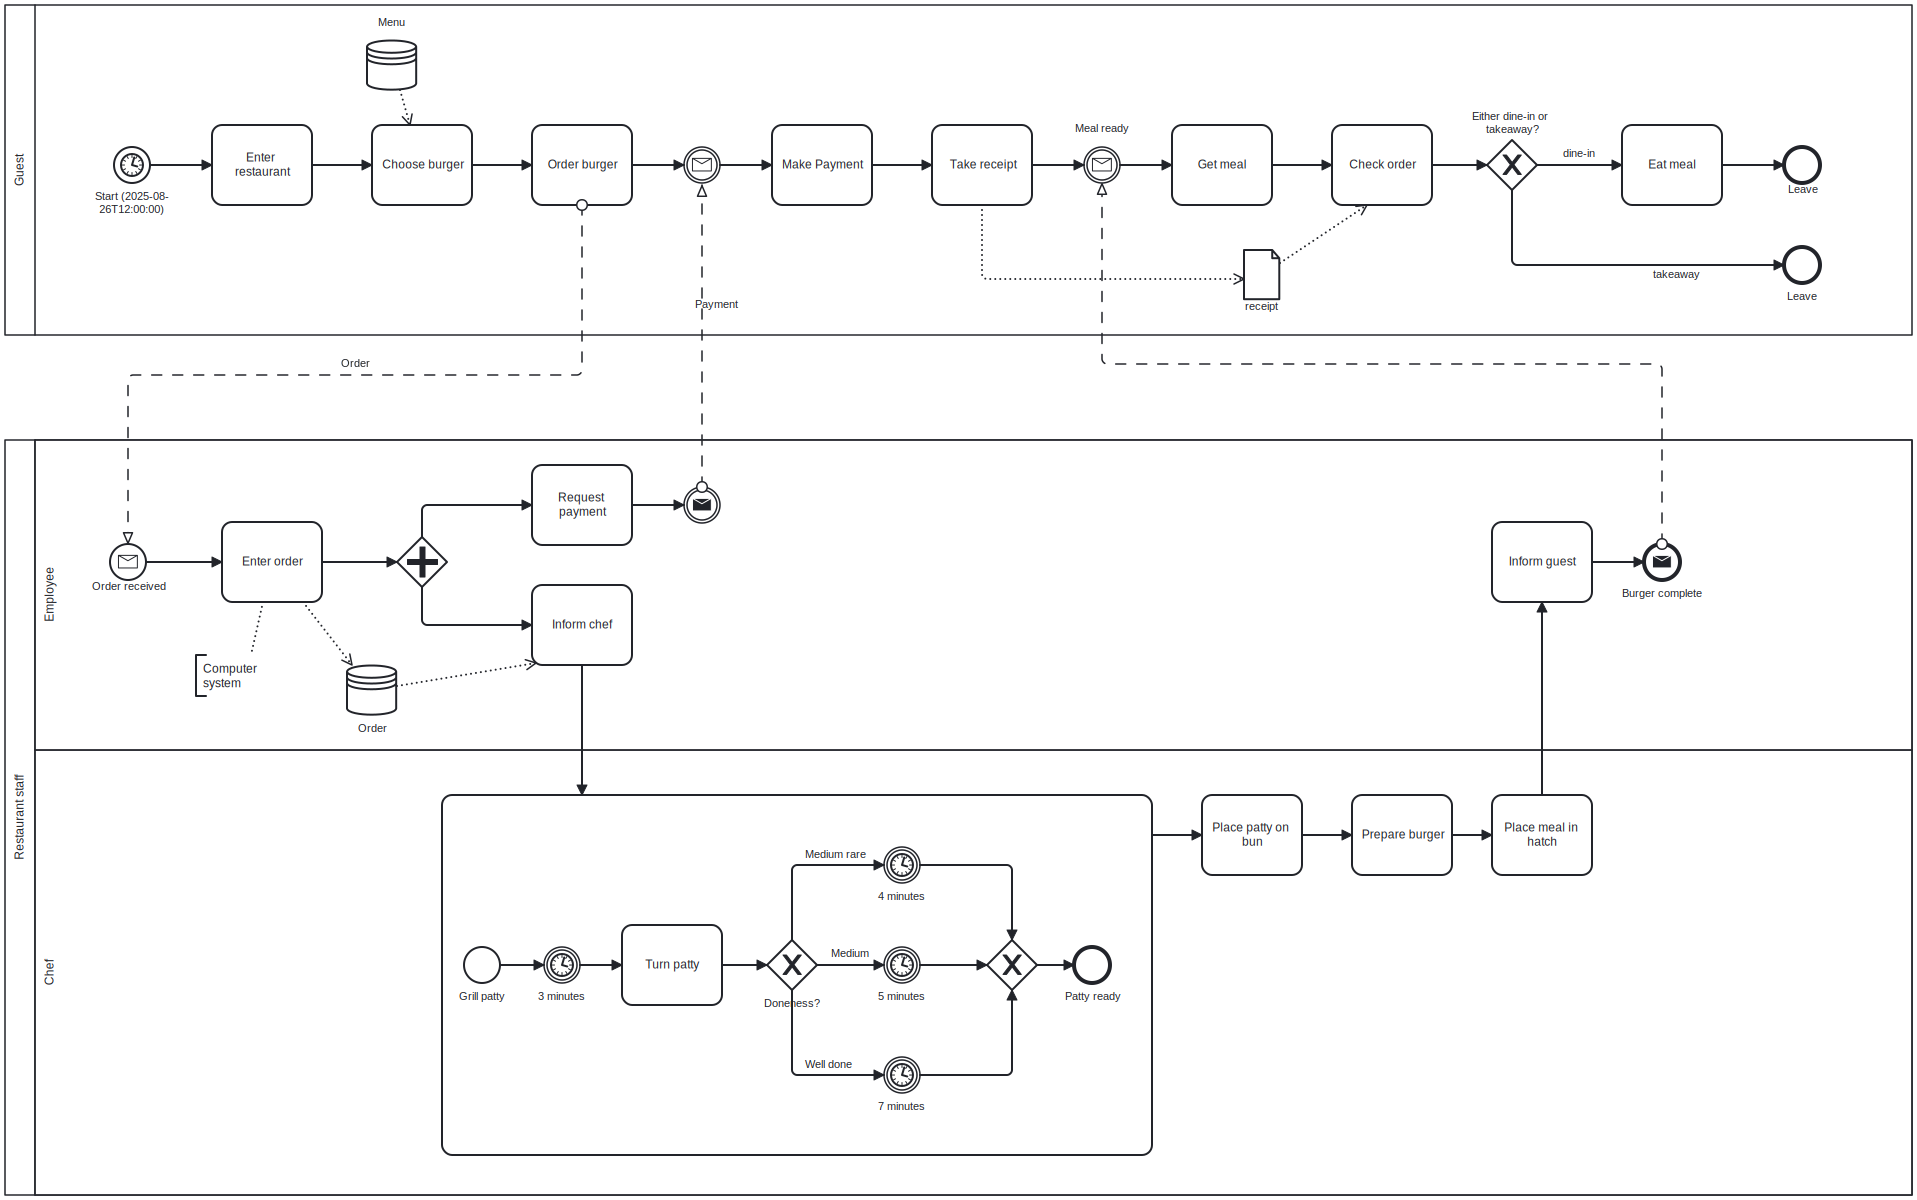
\includegraphics[width=\textwidth]{images/diagrams/diagram_0}
    \label{fig:bpmn-elements}
    \caption{BPMN 2.0 Diagramm mit allen relevanten Elementen}
  \end{figure}


Für die Chatbot-Implementierung ist das Verständnis dieses Systems entscheidend, 
da alle Elemente diesen Konventionen entsprechen müssen, damit sie 
in bpmn.js korrekt dargestellt werden. 


\section{Large Language Models}

Large Language Models (LLMs) sind Systeme, die auf der Verarbeitung und Generierung 
natürlicher Sprache spezialisiert sind. 
Sie basieren auf \texttt{Deep-neural Networks}, insbesondere auf Transformer-Architekturen, die große 
Mengen an Textdaten analysieren, um Muster, Strukturen und Zusammenhänge in der Sprache zu erkennen. 
Durch dieses Training können LLMs sowohl Texte verstehen als auch neue Texte generieren.

Ein LLM wird typischerweise durch überwachtes Lernen trainiert, wobei 
das Ziel darin besteht, das nächste Wort oder den nächsten Satz in einem gegebenen Kontext korrekt 
vorherzusagen. 
Moderne LLMs, wie GPT-Modelle, verfügen über Milliarden von Parametern, die ein 
Sprachverständnis und die Fähigkeit zur Textgenerierung besitzen.

Die Anwendungsbereiche von LLMs sind vielfältig. Sie reichen von Textgenerierung, Übersetzungen und 
Zusammenfassungen über Frage-Antwort-Systeme bis hin zu Chatbots und automatisierten 
Prozessunterstützungen. 

LLMs können genutzt werden, um Geschäftsprozesse in BPMN-Diagramme zu überführen. 
Dazu analysiert das Modell natürliche Sprache, wie z.B. Prozessbeschreibungen, 
Anweisungen oder Anforderungen, und 
wandelt diese in strukturierte BPMN-Elemente wie Tasks, Events, Gateways, Pools und Lanes um. 
LLMs können dabei sowohl die logische Abfolge der Prozessschritte erkennen als auch Verzweigungen 
und Kommunikationsflüsse zwischen Beteiligten identifizieren.

In der Praxis erfolgt dies oft in Form einer Text-zu-BPMN-Übersetzung, bei der das LLM die 
Prozessinformationen in eine JSON- oder XML-Repräsentation überführt, die anschließend von Tools 
wie bpmn.js visualisiert werden kann. 
Auf diese Weise können LLMs die Erstellung von Prozessmodellen erheblich beschleunigen, 
Standardisierung fördern und auch komplexe Abläufe automatisch konsistent darstellen.

\section{Chain of Thought}

Chain of Thought beschreibt eine Methode, bei der ein Large Language Model (LLM) seine 
Gedankenschritte offenlegt und erklärt, wie es zu einer bestimmten Antwort kommt. 
Statt nur ein Ergebnis zu liefern, zeigt das Modell also den Weg dorthin, ähnlich wie ein Mensch, 
der seine Überlegungen laut ausspricht. 
Diese Vorgehensweise ist besonders hilfreich bei Aufgaben, die mehrere Denkschritte erfordern, 
etwa beim Lösen von Problemen, beim Strukturieren von Informationen oder beim Verstehen komplexer 
Anweisungen.
Diese Vorgehensweise wurde von Wei et al.\ grundlegend untersucht
~\cite{wei2023chainofthoughtpromptingelicitsreasoning}.

Im Kontext der Unterhaltung zwischen Mensch und KI führt Chain of Thought dazu, dass das Modell 
transparenter und nachvollziehbarer reagiert. 
Die KI kann Gedankengänge ausformulieren, Entscheidungen begründen und schwierige Themen Schritt 
für Schritt erklären. 
Dadurch entsteht ein natürlicherer Dialog, da der Benutzer nicht nur das Ergebnis sieht, sondern 
auch versteht, wie die KI dorthin gelangt ist. 
Gleichzeitig hilft diese Technik dem Modell selbst, bessere Antworten zu geben, weil es 
Zwischenschritte bewusster berücksichtigt und Fehler eher vermeiden kann.

Für die Erstellung von BPMN-Diagrammen ist diese Vorgehensweise besonders wertvoll. 
BPMN erfordert eine klare Struktur von Ereignissen, Aufgaben, Gateways und Abläufen. 
CoT ermöglicht es ChatGPT, Prozessbeschreibungen in einzelne Handlungsschritte zu zerlegen, diese 
sinnvoll anzuordnen und anschließend die passenden BPMN-Elemente daraus abzuleiten. 
So lässt sich Schritt für Schritt erarbeiten, welche Tasks benötigt werden, wo Entscheidungen 
auftreten und wie die Kommunikation zwischen Rollen oder Abteilungen abgebildet werden muss. 
Chain of Thought macht die Diagrammerstellung dadurch deutlich präziser, transparenter und 
konsistenter.

\section{Streaming}

\section{Base64}

\section{Reflective Prompting}

